%\documentclass{../_combined/fcg-book}
\chapter{Preview}

\setcounter{foot}{1}
When people see the Talking Heads for the first time, they 
are stunned. It takes a while before
one gets used to the self-generated movements of each robot, 
the strange dialogs in an incomprehensible language, 
the graphs plotting the evolution of their internal
states, 
and the colourful environment which is the subject of their 
language games. But after some time, almost everyone gets involved 
in the game and attempts to figure out the language the robots
have developed or to teach them his own. 
Some people come back
day after day to follow the progression
of the language and conceptualisations that the Talking Heads 
build in collaboration with interacting observers.
Children are the first ones to 
start playing with neither fear nor preconception. 

This chapter explains the general setup of the 
experiment and gives a rough idea of what is going on. 
The various principles and mechanisms at work 
will be discussed in more detail later and I will also give many 
more examples taken from concrete interactions.

\section{The Main Components}

Clearly in the development of language and meaning, 
the group and the environment matter. A child 
who grows up without a caring 
community or without sufficient environmental stimuli
never develops the rich cognitive capacities 
normal adults have. From attempts to educate `wolf children'
who grow up in isolation from a human community, or 
impaired children for whom the intensity of early 
interactions are limited, we know that 
there are critical periods
where a community and a challenging environment must be
present otherwise the child's capacities for language
are damaged for the 
rest of his or her life.\footnote{See \cite{Tager:1994}.}

But how can we sufficiently 
recreate these social conditions in experiments 
with artificial systems? 
Building colonies of physical autonomous robots
roaming the world in search of stimulating 
environments and rich interactions with
other robots is not feasable today. So how 
can we ever test seriously situated and 
socially embedded approaches to cognition? 

\subsection{Teleporting}

Let me make a distinction between the physical aspects of 
a cognitive agent and the mental aspects. The physical aspects include the 
agent's body, the sensors and articulators, 
the physical location, the objects in this location, and the other
agents physically present in the environment. The 
mental aspects include the agent's repertoire of behaviors, 
the brain structures and processes
performing categorizations of reality, his
memory, lexicon, grammar, and so on. 
In the case of humans, these two aspects are intimately 
connected and indivisible. We cannot teleport our mental 
faculties into another body, or into another copy of 
our body, even though there have been speculations that 
we could in the future record human 
brain states,\footnote{
Such visions of the future have been put forward
by Hans Moravec \cite{Moravec:1995}. Neither current artificial intelligence technology nor
the state of the art in brain state recording are anywhere 
near to realising these visions.}
I believe that this will still not enable teleportation
because in human brains there is no distinction between 
hardware and software. The architecture of a human brain, 
the physical connections between cells, and the 
biochemical processes in each cell determine the brain's behavior.
There is no separation between a `brain program' and
an interpreter that reads brain programs and 
executes them. The brain is a special-purpose 
hardware device which is unique to each individual. 
To copy such a device we would have to rebuild it physically,
atom by atom, and integrate it in an exact copy of the 
same body. 

\begin{figure}[htbp]
  \centerline{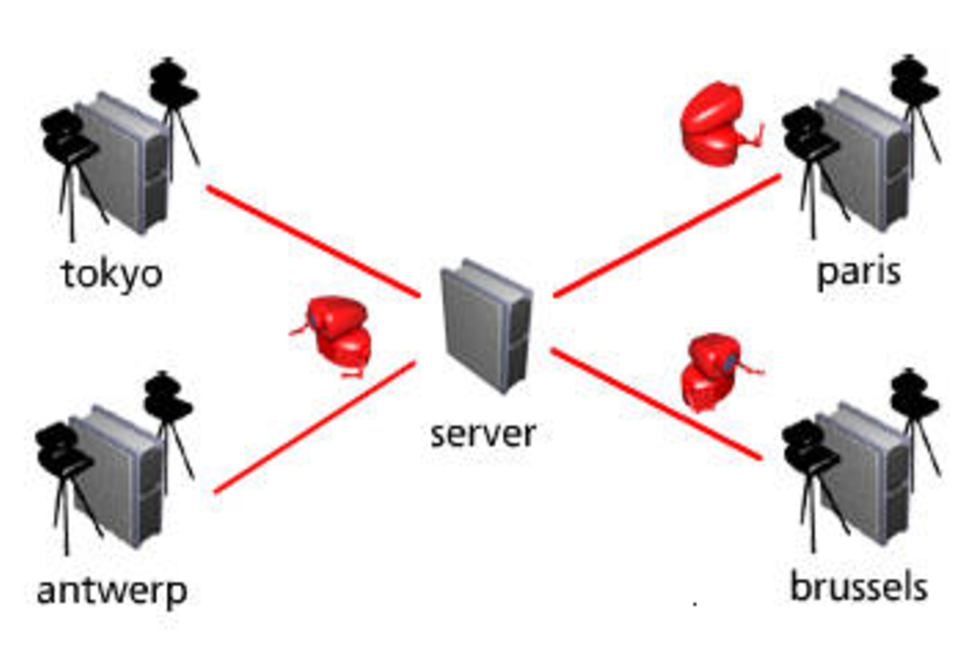
\includegraphics[width=.50\textwidth]{chap1/figs/teleportation}}
\caption{ The Talking Heads agents are implemented as software entities that can travel over the internet. 
To play a game, they get downloaded in a local server that drives the cameras and orchestrates a game. After a game, the software 
state is uploaded again to travel towards another location.}
\label{f:teleport}
\end{figure}

However, in the case of computer-based \is{teleportation}
artificial agents, we {\it can} 
make the distinction. It is possible to capture the mental state
of an agent in software, load this into a physical 
body, and then operate 
the agent. Afterwards the agent can extract himself
again from the body, teleport himself 
to another physical location through a data transmission network
like the Internet, get instantiated there in another
body, and experience another reality and physically meet
other agents. This is exactly how we have implemented the 
Talking Heads experiment.\footnote{
The agent teleportation infrastructure is in itself a 
fascinating non-trivial engineering project. Contributions 
from Angus McIntyre, Alexis Agahi, Sylvere Tajan and
Frederic Kaplan are gratefully acknowledged \cite{McIntyre:1999}. 
The fact that agents can teleport proves that we are dealing 
with a truly distributed multi-agent system. It also 
introduces physical parallelism in the agent-agent and 
agent-environment interactions. 
For a general introduction into multi-agent system
technologies and design methodologies, 
see \cite{Ferber:1999}.}
There are on the one hand
the physical structures, which I will refer to as the {\it
robot bodies}. They are installed in different physical 
locations somewhere in the world and connected
with each other through the Internet. Then there is 
a population of software structures that 
are occasionally loaded and instantiated in specific
robots. I will call these software structures
{\it virtual agents}. 
A {\it real agent} (a Talking Head) 
only exists when the virtual agent is
loaded in a physical robot body. 

Virtual agents cannot interact and 
an interaction between two `real' agents
can only take place when they are both physically present
in the same location. Thus an agent can travel from
Paris to Tokyo at the blink of an eye, rather than having
to take a plane, but two agents can only interact when they
are instantiated in the same physical environment. 
It is in principle possible that agents in different 
physical locations describe to each other the environment that they 
see (but which the other one does not see), just as we 
would do in a telephone conversation. This is only possible,
however, after the agents have had sufficient interactions
with each other in a shared physical world to have 
developed and learned a grounded shared language. 

The teleporting setup enables some fascinating 
experiments, engulfing the 
whole globe. The same agent can look at a scene from
different points of view or at scenes in different
physical locations in the world by teleporting himself in different 
bodies. He can develop categories in one location
and enrich his learning experience by moving to a new 
location which has different objects and thus poses new 
categorial challenges.
There can be populations of varying sizes with new 
agents being born and older agents dying, just like in 
natural human populations, so that we can study the 
transmission of language from one generation to the next
or the resilience of a language against an influx and 
outflux of agents. We can also let agents develop in
different parts of the world and have them migrate to
study intercultural exchange and language contact. 

\subsection{The robots}

A blind person who receives sight after the critical 
period for acquiring visual categorization undergoes a 
traumatic experience, \cite{Zeki:1993}. 
We could in principle build robot bodies
through which agents can experience their world with tactile
sensing and other robot bodies which support visual sensing, or both. 
But then an agent which had only access to tactile
sensing might suddenly find himself in a body equiped with 
vision. This pathological complication will 
be avoided by using the same robotic infrastructure
in every location, even though it would be fascinating and 
technically possible to study multi-modality in its 
own right. 
We also decided to make the robots vision-based, because visual 
sensing is one of the major sources of meaning in
human natural languages. 

Concretely, each robot consists of five building blocks (see \figref{f:plate2}):
\begin{itemize}
\item A camera mounted on pan/tilt motors so that it can move 
up or down and left or right. 
\item A loudspeaker (for voice output) and a microphone (for 
voice input). Each agent has a particular quality of voice
output with male and female voices, so that it is possible 
to keep them apart in the dialog. 
\item A computer that can house an agent's 
cognitive architecture as well as peripheral 
control software to steer the movements of the camera, 
receive and preprocess images, or synthesise and analyse 
sound. This computer is connected 
to the Internet to allow virtual agents to be loaded and instantiated. 
\item A television screen that shows {\it us} what the agent
instantiated in a body currently sees through the camera. 
\item A computer screen that shows {\it us} what is going on inside
the brain of the agent currently installed in the robot (\figref{f:agentview})
\end{itemize}

\begin{figure}[htbp]
  \centerline{\includegraphics[width=.60\textwidth]{chap1/figs/interface.pdf}}
\caption{ Interface through which the internal states of agents can 
be inspected. Two agents are shown. The top windows show the state of an agent, 
the middle windows the camera inputs that the agent sees and the bottom windows show 
their discrimination trees.}
\label{f:agentview}
\end{figure}

In constructing the robot bodies, we have used as much as
possible off-the-shelf standard 
components so that we could focus almost completely on issues
directly relevant to language and meaning.
Each robot's low-level vision system
(integrated in the camera) is already very sophisticated.\footnote{
The camera is a Sony EVI-D31. The main computer is a Power 
Macintosh from Apple, Inc. The agent servers run under the 
Lynux operating system.}
It can focus automatically to get a sharper image
and autonomously track a moving object. The speech signal is 
produced with a standard text-to-speech system 
so that we did not have to 
worry about building complex audio modules ourselves.
The computer hardware 
is powerful, but not specialised nor in the supercomputer 
range. All programs have been written in the standard symbolic 
programming language of artificial intelligence 
research, namely LISP.\footnote{
The construction of the programs underlying the 
Talking Heads experiment has required advanced
artificial intelligence programming techniques, 
such as discussed by \cite{Norvig:1996}. A general
toolkit for the systematic execution of 
simulation and physical experiments, called BABEL, has been
designed and implemented by Angus McIntyre. The 
toolkit allows the definition and modular composition
of cognitive architectures, the design of 
experiments, and the monitoring and displaying of 
results, \cite{McIntyre:1998}.} What makes the Talking Heads experiment
special is not the hardware or software tools
but what we have done with it.

\subsection{The agents}
\is{agent}

Agents can only engage in interactions with other agents 
when they are physically instantiated
in a robot. Each agent has a basic brain architecture
with different layers performing the cognitive functions 
relevant for playing language games: 
\begin{itemize}
\item A perceptual layer which performs low level signal 
processing to segment the image and collect data about 
each segment such as the colour, size, position or shape
of a segment. 
\item A conceptual layer which categorizes and 
conceptualises the segmented and processed image. 
It is based on a self-generated and evolving repertoire
of categorial distinctions, such as red versus green, or
small versus large. Such a repertoire is referred to as 
the agent's ontology in this book. 
\item A lexical layer which maintains an evolving repertoire
of associations between meanings and words, which I will refer to 
as the lexicon, and performs lexical lookup while parsing 
or producing utterances. 
\item A syntactic layer which uses 
grammatical schemata for organising words
in larger structures or for recognising these structures and
reconstructing complex meanings. 
\item A pragmatic layer which carries out the
scripts for playing language games and maintains the machinery 
for engaging in interactions with other agents in a 
shared environment. 
\end{itemize}
Each of these layers is described in more detail 
later. The internals of the layers are not static but
constantly evolving and adapting. They are not strictly 
modular but coupled in various ways to each other.
Each verbal interaction 
in effect changes the agent's internal state and thus 
influences future behavior. A new, virgin agent 
starts without any built-in ontology, lexicon, nor grammar. 
This is one of the crucial points of the whole experiment, 
because we want to test possible theories on how language
and meaning can evolve and be acquired {\it ab initio}. 

Agents are part of populations which determine the probability
with which they encounter each other. This generates 
a dynamic process at two levels: There is the dynamics of the evolving
cognitive competence of each agent (the ontologies, 
the lexicon, the grammar), and there are 
the evolving macroscopic structures which arise in a population
of agents, such as the common lexicons or shared grammars. 
We will see that the mental 
characteristics of agents, even in a single population, are never 
identical because each agent has his own history of 
interactions with the environment and with other agents. 
This is another crucial aspect of the experiment. 
We want to investigate in how far communication is possible
without complete ontological or linguistic coherence. 

\subsection{Interactivity}

To qualify as a sound scientific experiment, anybody 
who wishes to challenge the claims should be given 
the tools `to see for himself'. There are three 
ways in which we have empowered observers to do so. 

First, each physical Talking Heads site has 
a complex infrastructure to organise the interactions between
agents operating in that location, and to support the
arrival and teleporting of agents. This infrastructure also houses
a {\it commentator}, a computer program that
monitors the dialogs, inspects the internal states of each
agent, and displays useful statistics such as the degree
of sharing of the lexicon, the competition between different
words to express a particular meaning, the stability of 
certain syntactic constructions, etc. The commentator 
produces spoken or written comments and displays
measurement results on an additional computer screen. 

Second, the teleporting infrastructure makes it possible 
to implement interactions between humans and artificial agents, 
either directly in the shared physical environment or 
through the Internet. At any time, a human experimenter can
pretend to be one of the agents: seize 
a robot, partly control the
camera to set the context of an interaction, and type 
in expressions playing the role of speaker or hearer in 
a language game. The human experimenter can create a 
new, virgin agent, track in detail how this agent acquires the 
categories and language in an existing group, 
or try to influence the currently dominating language
by introducing new words or constructs and following
their propagation (see \figref{f:plate8}). 

\begin{figure}[htbp]
  \centerline{\includegraphics[width=.80\textwidth]{chap2/figs/interface}}
\caption{ Internet interface through which users can 
access the state of games on remote sites and 
follow the experiment.}
\label{f:plate8}
\end{figure}

Finally, the environment has been restricted to 
increase the transparency of experimental results. It 
consists in all locations of a magnetic white board mounted
on the wall in front of the robots (see \figref{f:plate9}). On this
board, the human experimenter can paste various
figures, typically stylised geometric figures like 
rectangles, circles, and squares,
in various sizes, shapes and colours. By changing the 
environment, the experimenter can try to find out what
visual categories the agents employ and force the expansion 
of categorial repertoires, for example by pasting
new types of figures on the board. He can probe the 
adaptivity of the agents by setting up situations that 
destabilise an existing lexicon and see how long it 
takes before a new, perhaps more abstract lexicon emerges. 
All these tools generate unprecedented opportunities to apply 
the most rigid scientific evaluation criteria to the
theories of language and cognition that I will propose in this
book. 
\begin{figure}[htbp]
  \centerline{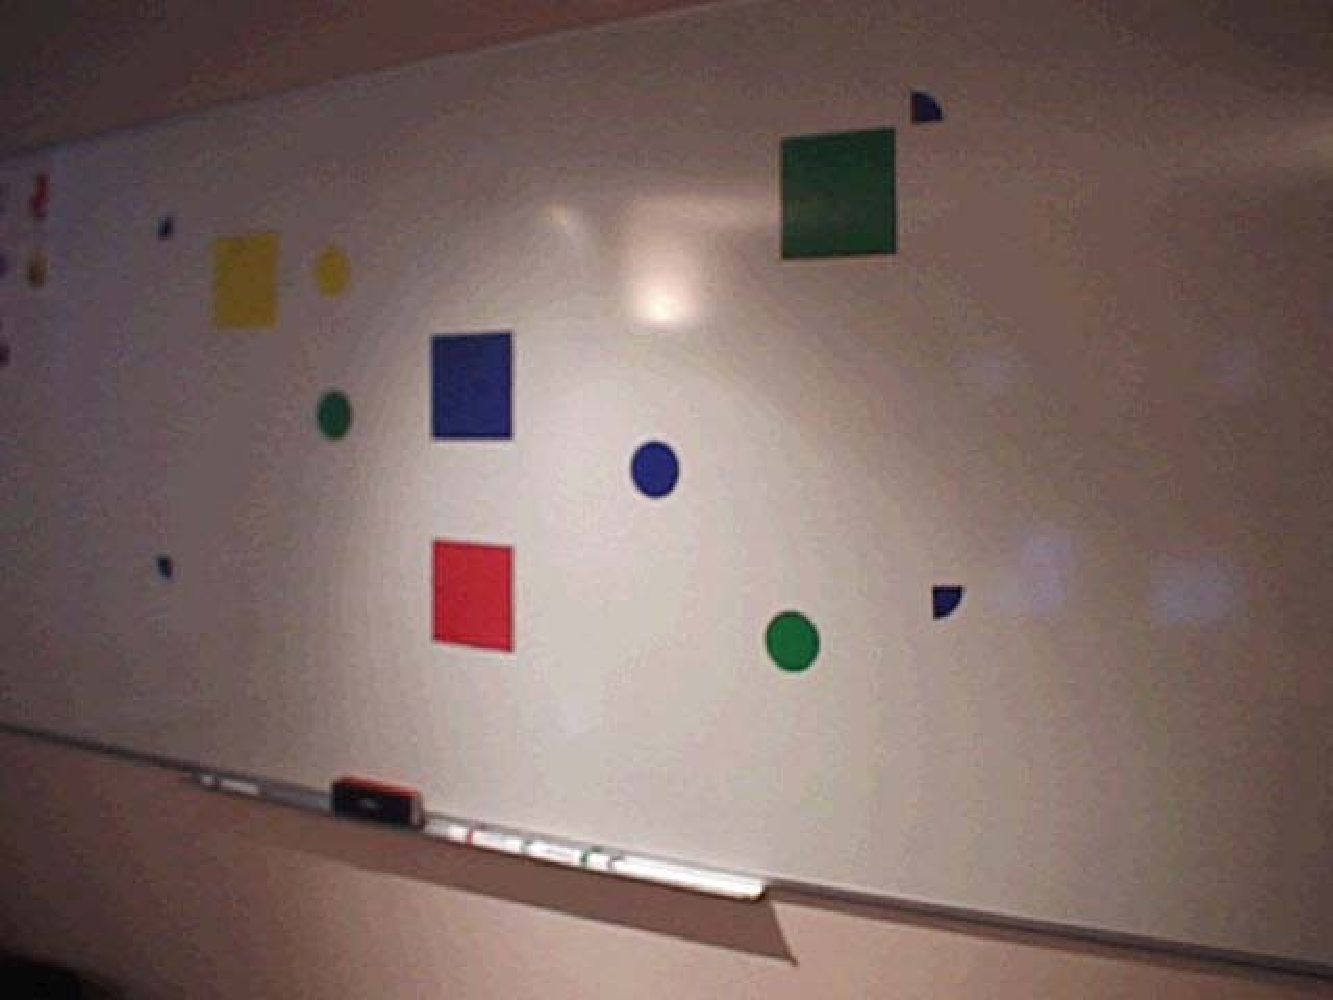
\includegraphics[width=.60\textwidth]{chap1/figs/Whiteboard}}
\caption{ The physical environment of the Talking Heads  
consists of a white board on which various
geometric figures can be pasted. The light conditions were not under the control 
of the experimenters in most locations.}
\label{f:plate9}
\end{figure}

\section{The Guessing Game}

Given this rich computational and robotic infrastructure, many \is{Guessing Game}
specific experiments are possible. 
Each experiment could explore
a particular interaction between the robots, the environment, 
and human observers. In this book, I explore only 
one type of interaction, which I call the
{\it guessing game}.\footnote{
A very similar game has been called the original 
language game by \cite{Brown:1973} in the context of
research on child language acquisition. See also 
the thoughtful analysis in \cite{Halliday:1975}. 
Research on child language has inspired the 
agent architectures and behaviors but they should not
be seen as a realistic model of child language acquisition.}
The Talking Heads play this game 
either among themselves or with a human experimenter. 

\subsection{Rules of the game}

The guessing game is played between two 
physically instantiated agents. Agents in 
a virtual state must queue up to have access to one of the 
robot bodies installed in a particular site before
they can play the game. One agent 
plays the role of {\it speaker} and the other then plays the 
role of {\it hearer}. Agents take turn playing games 
so that all of them develop the capacity to be speaker or hearer.
A human experimenter can pick one of these roles and 
play the game instead of an artificial agent. 

The speaker first looks at one area of the white board and 
directs the attention of the hearer to the same area.\footnote{
I will explain later how exactly agents
decide on a particular scene and how they are able to 
draw each other's attention to specific areas of the 
white board.}
The objects located in this area constitute the {\it context}. 
The speaker then chooses one object from the context, which 
I will call the {\it topic}, and gives a verbal hint
to the hearer. The {\it verbal hint} is an expression
that identifies the topic 
with respect to the other objects in the context. For example, 
if the context contains a red square, a blue triangle, 
and a green circle, then the speaker may say something like 
"the red one" to identify the red square as the topic. 
If the context contains also a red triangle, he has to be more 
precise and say something like "the red square" to delineate
the topic from the non-squares as well as
from the blue square. 
Of course, the Talking Heads do not say "the red square"
but use their own language and concepts which are not 
necessarily the same as those used in English. For example, 
they may say "malewina" to mean [UPPER EXTREME-LEFT LOW-REDNESS]. 

Based on the verbal hint, the hearer tries to guess what
topic the speaker has chosen, and communicates his choice 
to the speaker by pointing to the object. Given that 
the robots do not have arms, pointing is realised by 
focusing on an object. One robot can `see' in which direction another one 
is looking, and thus know where he is `pointing'. 
The game succeeds if the topic guessed by the hearer is 
equal to the topic chosen by the speaker. 
The game fails if the guess was wrong or 
if the speaker or the hearer failed at some earlier point in the 
game. 

In case of a failure, the speaker gives an extra non-verbal
hint to the hearer by himself pointing to the topic, 
and both agents try to repair
their internal structures to be more successful in future
games: The speaker weakens his hypothesis that the words
and constructions he used 
were `right', in the sense of shared by other agents. 
The hearer tries to guess what meanings the speaker 
might have used and deduce what form-meaning relations or 
syntactic constructions he is missing. Pointing by gesturing is
always vague, and the repair actions are far from guaranteed to succeed. 
Nevertheless, they gradually lead (as we will see) to 
a sufficiently shared communication system meaning that 
success in guessing the topic purely based on language
communication increases to reach almost 100 \%. 

\subsection{Nature of the game}

The Guessing Game is one of the common things we do with language. 
For example, I play a similar game when I sit with a friend
at the dining table and say "could you give me the salt". 
If she guesses correctly what I mean and hands 
me the salt, the game has succeeded. If she looks at me 
with a puzzled face (maybe she does not speak English) or hands me
the salmon instead of the salt, the game has failed. In that case, 
I can gesture in the direction of the salt and say "no, no, the {\it salt}
please", and perhaps then she hopefully realises and gives the salt to me. Failure 
is common in natural language dialogs and may be caused by 
many factors. For example, the salmon could indeed 
be close to the salt and my pronounciation of the word "salt"
may have sounded a bit like "salmon", perhaps because there was
loud music playing in the background or perhaps
my friend does not understand English. 
A failure is often 
an opportunity to negotiate how something will be expressed
in the future. For example, the hearer may pick up a new word
or the speaker may realise that a certain word is 
not appropriate in this particular context. 

The guessing game is not a game of winners and losers because both 
agents win or both agents lose at the same time. But it is a game
nevertheless, because it is played with clear rules, 
with a clear outcome and strict limitations on how 
success can be achieved. An agent can not look inside another
agent's brain state. Agents can only interact through the 
external environment. There is no global control 
center that is monitoring the behavior and internal states
of all agents and setting the way they should speak or 
perceive their world. The artificial agents are autonomous and
fully distributed, just like human beings. 

The game is different from a closed world game like 
chess, because the environment is open. The human 
experimenter may introduce new objects at any
time, any one agent can extend
the language (for example invent a new word), possibly
requiring the other agents to adopt it as well, or the
human experimenter may inject new language forms in the 
dialogs. Agents try to maximise their communicative 
success so they cooperate to the fullest and update or change
their internal structures and processes
to improve their chances in the game.\footnote{
The guessing game is a cooperative game, because
both the agents win or loose at the same time and have 
the highest gain if they develop co-ordinated behavior. 
The agent who manages to have most success in the game is 
the global winner. Because the commentator requires to know 
from the speaker which topic he wants to communicate 
before he is allowed to speak, no cheating 
is possible. Game theory, originally founded by 
von Neumann and Morgenstern, can be applied to study the 
language game mathematically. \is{game theory} We are dealing with an 
evolutionary game in which the players optimise their 
internal states to become better in the game 
\cite{Maynard:1982}.}

In the Talking Heads experiment, it is assumed that 
agents want to cooperate and that they use communication
as part of their cooperation. 
The evolution of cooperative games has been studied 
extensively by artificial life researchers often 
in the context of Axelrod's prisoners dilemma game,\is{prisoners dilemma game} 
see for example: \cite{Ikegami:1994} 
For a general introduction how communication can 
evolve in the context of cooperation, see: \cite{Hauser:1996}. 
Computer simulations showing the evolution of 
cooperation and communication have been reported in the
artificial life literature. See for example: \cite{MacLennan:1991} 
Most of these computer simulations are 
closer to animal signaling systems than to human lexicons
both in size and in terms of the complexity of meaning.

The guessing game is clearly not the only thing we do 
with language. Humans are capable of playing a whole 
range of language games and inventing
new ones when the circumstances
require it; however, to do controlled experiments we need
to limit ourselves. The objective of the Talking Heads
experiment is not to cover the full range and complexity
of human natural language interaction but to examine with
objective precision a limited number of issues concerning
the nature of language and meaning. 

\subsection{The semiotic square}

The environment of the Talking Heads is 
not fixed. The human experimenter 
may change the position of objects, add new kinds of 
objects, or eliminate
others. Consequently a strategy of naming individual objects
will not work. It would lead to a proliferation of 
proper names and it would require the Talking Heads to
recognise objects, which is very difficult to do.\footnote{
For a thorough exposition of the difficulties of 
object recognition, see \cite{Ullman:1996}
Object constancy comes fairly late in the 
acquisition of a child's ontology, as Piaget's conservation
experiments have shown. Language probably plays an important
role in forming the notion of an object.}
Indeed, humans don't exclusively use proper names in 
natural language conversations 
either. We say "could you give me the red small square" as 
opposed to "could you give me $O143$". Natural language 
words like "red" or "small" name perceptually grounded categories
and syntactic structures indicate how they should
be combined and used to find the topic. The relation between 
a language expression and its referent is therefore 
always indirect. This is summarised
in the semiotic square (\figref{triangle}), which I will use throughout this book to 
help understand and analyse the nature of language communication. \is{semiotic square}
The semiotic square relates the four entities
involved in a verbal interaction: 
\begin{itemize}
\item An {\it utterance}, such as "small red square", which is 
transmitted as a physical 
signal from one agent to another one through the 
external environment. It is written between double quotes. 
\item A {\it meaning}, which consists of categories like [RED], [SMALL], 
or combinations of categories, like \{[RED] [SMALL]\}. Labels of 
categories are written in capital letters between 
square brackets. 
\item An {\it image segment}, denoted as $S143$, which is 
a segment of the image perceived through the camera.
\item A {\it referent}, like object $O143$, which is 
an entity in the real world. 
\end{itemize}

\begin{figure}[htbp]
  \centerline{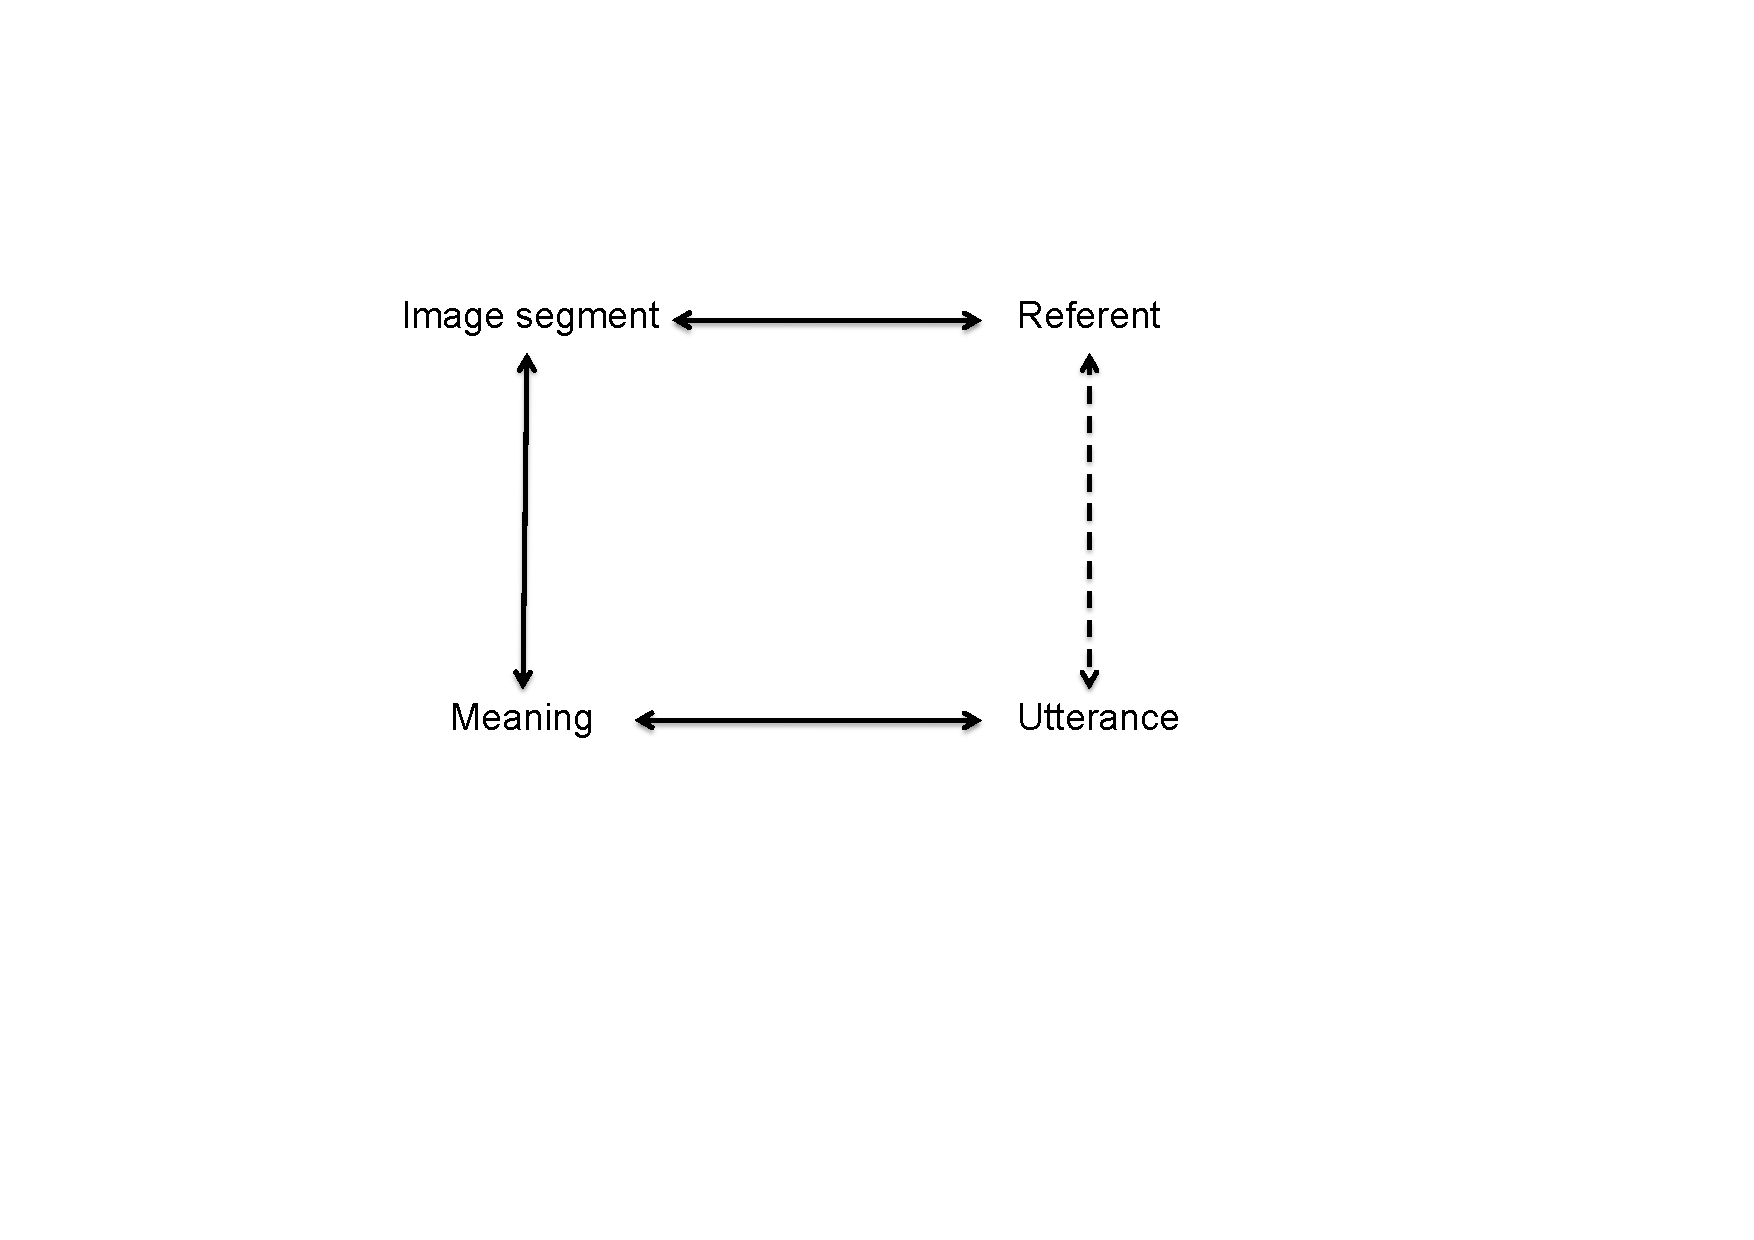
\includegraphics[width=.65\textwidth]{chap2/figs/triangle}}
\caption{\label{triangle} Any verbal interaction
involves four entities here grouped in the
`semiotic square'. The relation between utterance
and referent always needs to be established indirectly by 
passing through perception and meaning.}
\end{figure}

The systematic relation between meaning and referent is 
usually studied under the heading of semantics, and the 
systematic relation between meaning and utterance as
grammar (including syntax, morphology and lexicon).\footnote{
For a general introduction to the contemporary linguistic
viewpoint on the processes involved, see: \cite{Vanvalin:1997} 
In a logical approach to language, as 
exemplified by Montague grammar \cite{Montague:1974},  
meanings are represented using a logical formalism, i.c.
a variant of intensional logic. \is{Montague grammar}
Natural language expressions are systematically 
related to expressions in this logic, and a
formal semantics system defines how expressions in the logic
are mapped onto their denotations. Because this is 
a formal framework, the denotations consist of formal 
models. To make the Talking Heads experiment work, 
we needed to develop a grounded semantics system, which details
how an agent may go from physical reality to meaning
using a perceptual apparatus, and from meaning 
to physical reality. The logical structure of 
the meanings we will investigate are very simple 
(unary predicates and conjunctions). But once we know how to 
set up a grounded semantics for simple meaning
structures we can scale it up to the more complex meaning
structures typically studied in logic.}

Many tricky philosophical issues are raised in 
the unavoidable distinction between the sensed image
of an object (which is local to the agent)
and the object itself (which is external to the 
agent). Some philosophers even doubt that objects 
have an existence outside our perception of them! 
We need to make the distinction because agents always
have different internal images even if they look at 
the same object seen from our viewpoint as an external
observer. However, for simplifying the 
explanations, I will sometimes assume that perceived
image and external object are the same, so that the 
semiotic square becomes a semiotic triangle.\footnote{
The notion of a semiotic triangle was first
introduced in a classic of the semiotic literature, 
see \cite{Ogden:1935}.}

When we put together the semiotic squares of two 
agents (\figref{triangle2a}), we see more clearly 
that agents are trying to agree about a common object
in the external word, but they never have 
any direct access and hence confirmation whether they 
are really referring to the same object. 
Only through pointing or other
cooperative actions can speaker and hearer co-ordinate
whether they indeed refer to the same object in
the external reality. 

The utterance is not the same for both agents, because it
needs to be articulated, transmitted, and perceived through 
a physical medium. Errors in transmission or perception may 
and do occur and have an important impact on the evolution of 
language. To remain focused, I will not really treat this issue in 
this book but will instead assume that there is direct, error-free transmission
of the utterance. 

\subsection{Processes involved in language communication}

I will use the following terms for denoting the 
processes speakers and hearers go through while traversing
the relations in the semiotic square as they play a language
game (\figref{triangle2a}). 
A similar framework, but emphasising the 
language production side, has been described in great
detail by \cite{Levelt:1989}. That book also provides a wealth
of psychological evidence that these processes must 
be going on and expands the phonetic and phonological 
side. An example of a detailed architecture inspired by 
generative grammar is discussed in: \cite{Jackendoff:1997}. 
Generative approaches to language attempt to define a language by 
generating its set of possible utterances. Interpretations
are constructed from the syntactic structure derived by 
the generative grammar. In this book, we are interested 
in the mapping from communicative intent 
in a perceived reality to an utterance and back. The knowledge
and skill needed to solve this problem is different from 
that need to systematically generate the set of sentences in a 
language and their possible interpretations.

1. The speaker as well as the hearer {\it perceive} reality
by capturing an image through the camera, segmenting 
the image into coherent units, and deriving various 
sensory characteristics about each image segment, 
such as the colour, size, movement. 
\begin{figure}[htbp]
  \centerline{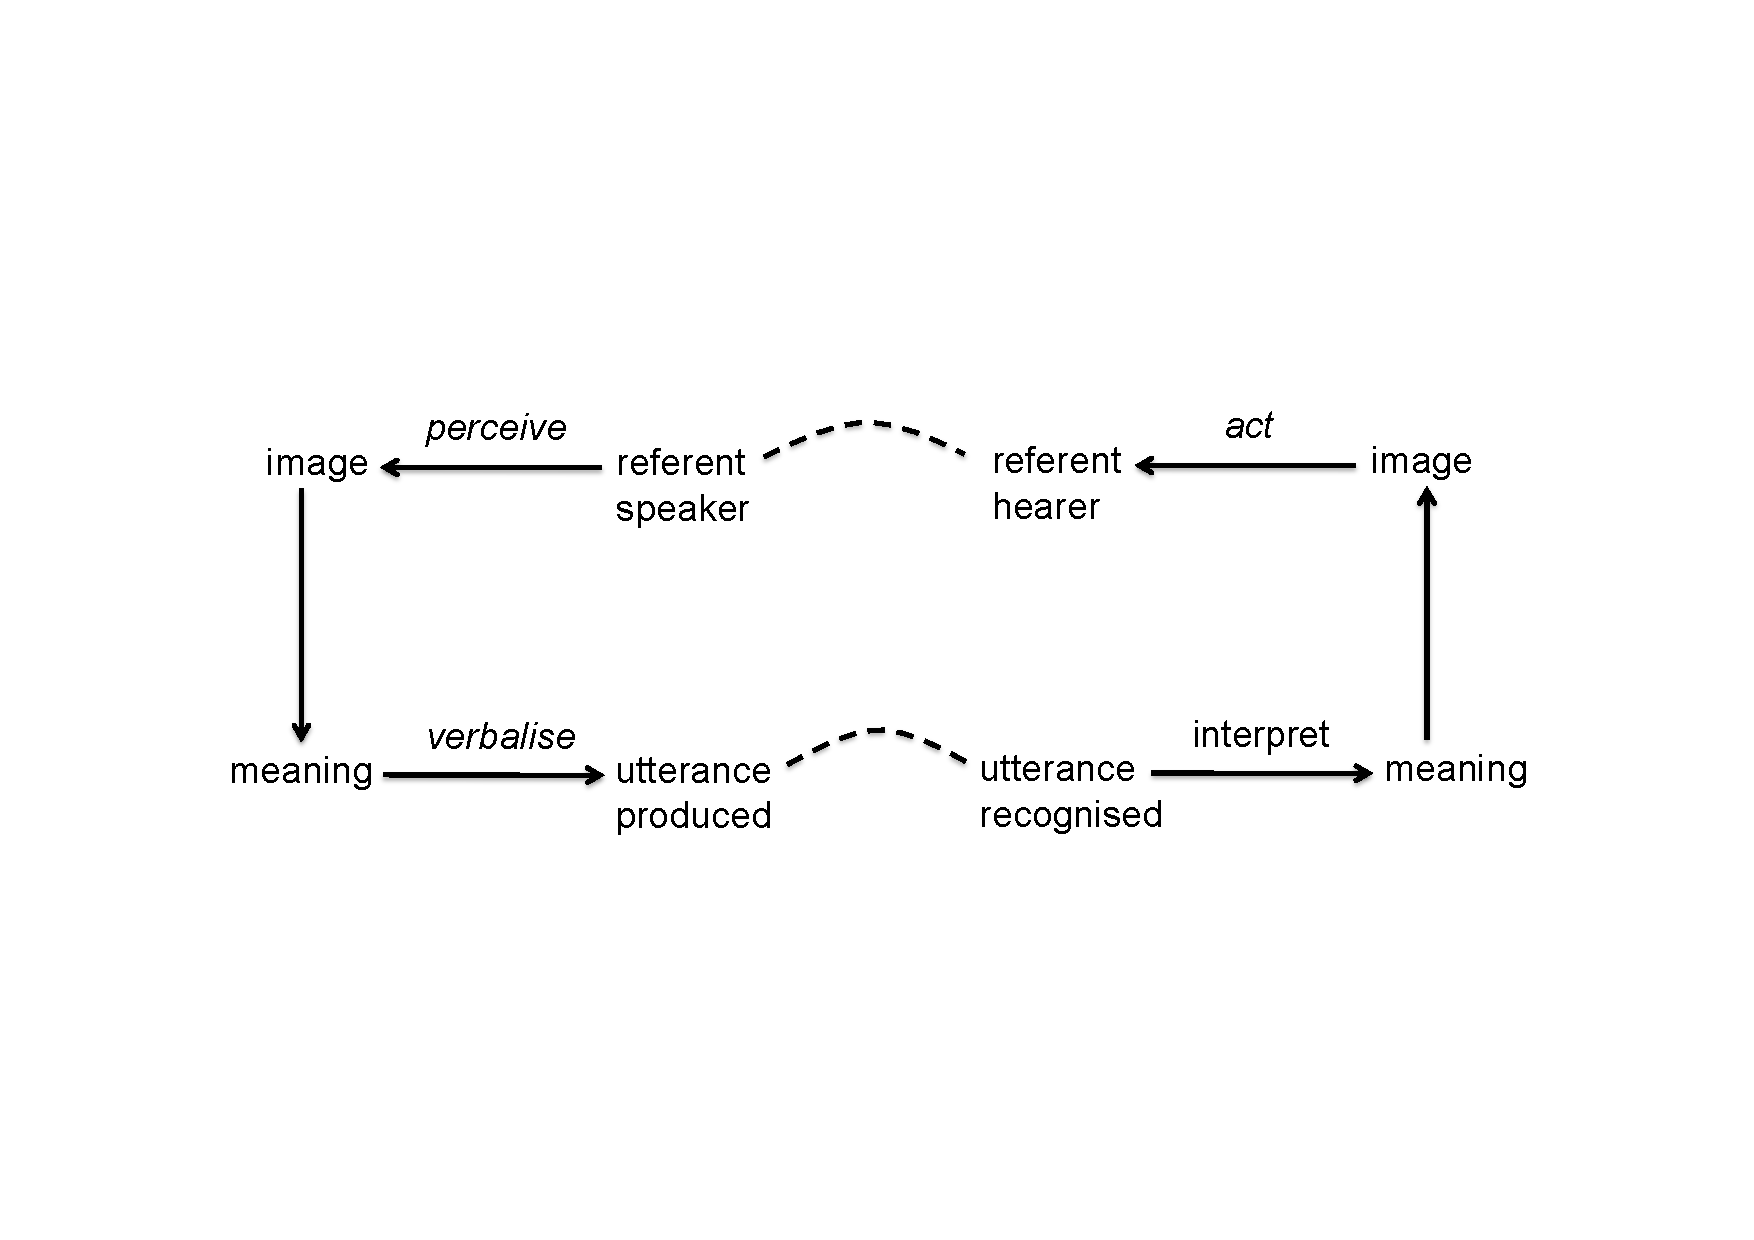
\includegraphics[width=.85\textwidth]{chap2/figs/triangle2}}
\caption{\label{triangle2a} Left: processes carried
out by the speaker. Right: processes carried out by the hearer.
There are also feedback processes moving in alternate directions
until the agents settle on coherent choices for all the items
in their semiotic squares.}
\end{figure}

2. The speaker must then {\it conceptualise} the 
scene on the basis of this perception. He must find a set of
categories or a conjunctive combination of 
categories that distinguishes the referent from the other objects in 
the context, and which will act as the meaning of 
his communication. For example, he might choose [BLUE] if the
topic has a blue colour and all the other objects in the 
context are not blue. 

3. The speaker must then {\it verbalise} this conceptualisation. 
He must use his language system to find words and 
syntactic constructions expressing this meaning.
For example, he might choose "blauw" (if he speaks
Dutch), or "bleu" (if he speaks French),
to convey the category [BLUE]. 

4. The hearer must engage in similar tasks but now
going in the reverse direction. He must
{\it interpret} the utterance to find out which
conceptualisation constitutes the meaning. 

5. Then the hearer must {\it apply} this meaning
to see what referent was intended. The hearer has
also perceived the scene in terms of a set of 
segments and now uses 
the meaning to identify the segment that
could have been the one intended by the speaker.

6. Finally the hearer {\it acts} upon the outcome of meaning
application. He points to the topic he has identified. This is the 
step where both agents co-ordinate their 
behavior through the external world. 

\subsection{Knowledge sources and competences}

Each of these activities requires knowledge and/or skill
(summarised in the table below). Perceiving requires 
visual processes capable of segmenting images and deriving image 
segments. Conceptualisation requires an {\it ontology}, 
a repertoire of perceptually grounded distinctions
that can be applied to a segmented image to yield 
distinctive categories or category combinations that 
may constitute the meaning of the utterance. Verbalising 
a conceptualisation requires 
a {\it lexicon} that maps parts of the meaning to words and 
a {\it syntax} that specifies how to organise individual words
into a larger complex. 
The hearer must use similar 
knowledge sources in the other direction. He must use 
his lexicon and syntax to reconstruct the meanings expressed
by the utterance, and then use the 
ontology again to apply the meaning to the present 
context to find the referent. 
\begin{center}
\begin{tabular}{| l | l | l | l |} \hline
{\it Activity} & {\it From} & {\it To} & {\it Knowledge source}\\ \hline
Perceive & Object & Image segments & Visual processes \\ \hline
Conceptualise & Topic & Meaning & Ontology  \\ \hline
Verbalise & Meaning & Utterance & Lexicon + syntax \\ \hline \hline
Interpret & Utterance & Meaning & Lexicon + syntax \\ \hline
Apply & Meaning & Topic & Ontology \\ \hline
Act & Topic & Object & Behavioral process  \\ \hline
\end{tabular}
\end{center}

I do not want to suggest that there is a simple linear flow 
neither from perception to utterance nor from utterance to 
perception. Instead, we must imagine a dynamic process 
involving forward and backward propagation of information 
until coherent choices for all the nodes in the two
semiotic squares have been established by the speaker and 
the hearer. Many different choices are initially possible 
(many segmentations, conceptualisations, verbalisations, 
interpretations) but the dynamic process gradually settles into 
a single coherent attractor, so that speaker and hearer 
agree upon a common referent. The co-ordination between 
chosen topic and identified referent is done through 
the real world (pointing, handing an object, performing
an action). 

I deliberately left an important aspect of language out. 
In the case of physical agents, the form cannot be transmitted
directly but needs to be articulated in speech sounds, 
written signs, or gestures, to create a true utterance. This additional 
complexity will not be discussed further in this book - even though 
it is a fascinating topic in its own right.\footnote{
See for a state of the art review: \cite{Clark:1990}
We have already been conducting quite extensive 
research in our group on the origin of sound systems 
using similar principles as the ones discussed in this 
book for the origins of word semantics. 
See: \cite{DeBoer:1997} The complex 
adaptive systems approach underlying this phonetics
work was already foreshadowed in work of phoneticians
like Bjorn Lindblom \cite{Liljencrants:1972}.}
To make a verbal interaction nevertheless complete, agents
are given a repertoire of consonants and vowels with 
which they can make random syllables and syllable combinations, 
like "wabido", "bimaku", etc. The articulation and 
recognition of these syllables is assumed to be acquired
already and transmission is engineered to be error-free. 
This way, our attention can be focused on how
ontologies, lexicons, and grammars may emerge. 

\section{Perception and categorization}

I will now discuss in some more detail each of the processes
the Talking Heads go through when they 
play a complete language game, leaving a more detailed 
discussion to subsequent chapters.

\subsection{Scene and topic selection}

Every physical Talking Heads set-up features a `waiting room' in 
which agents are stored, ready to be loaded into the 
robotic infrastructure or to be teleported to another
physical site. A game starts when two agents are chosen
at random from this waiting room and loaded into 
the two physical robots. The
internal architecture of each agent is connected with 
the sensori-motor apparatus of the robot so that they can 
receive the sensory data streams recorded by the camera
and control the movements of the robots. Then the general 
control system assigns randomly the role of speaker and hearer
to each of the agents and the game can begin. 

Next the speaker randomly moves around its camera, halts 
at a particular location, and captures
the image. The speaker then attempts to segment 
this image. If the scene is `interesting', which means that
there are at least two clear segments, it is chosen 
for playing a language game. Otherwise the agent makes another 
random movement and repeats the process. An example of 
an interesting scene with its subsequent segmentation
by the speaker is shown in \figref{f:plate10} (top image on the right). The scene
has two circles as main objects. Segments which are too 
small are ignored. 

\begin{figure}[htbp]
  \centerline{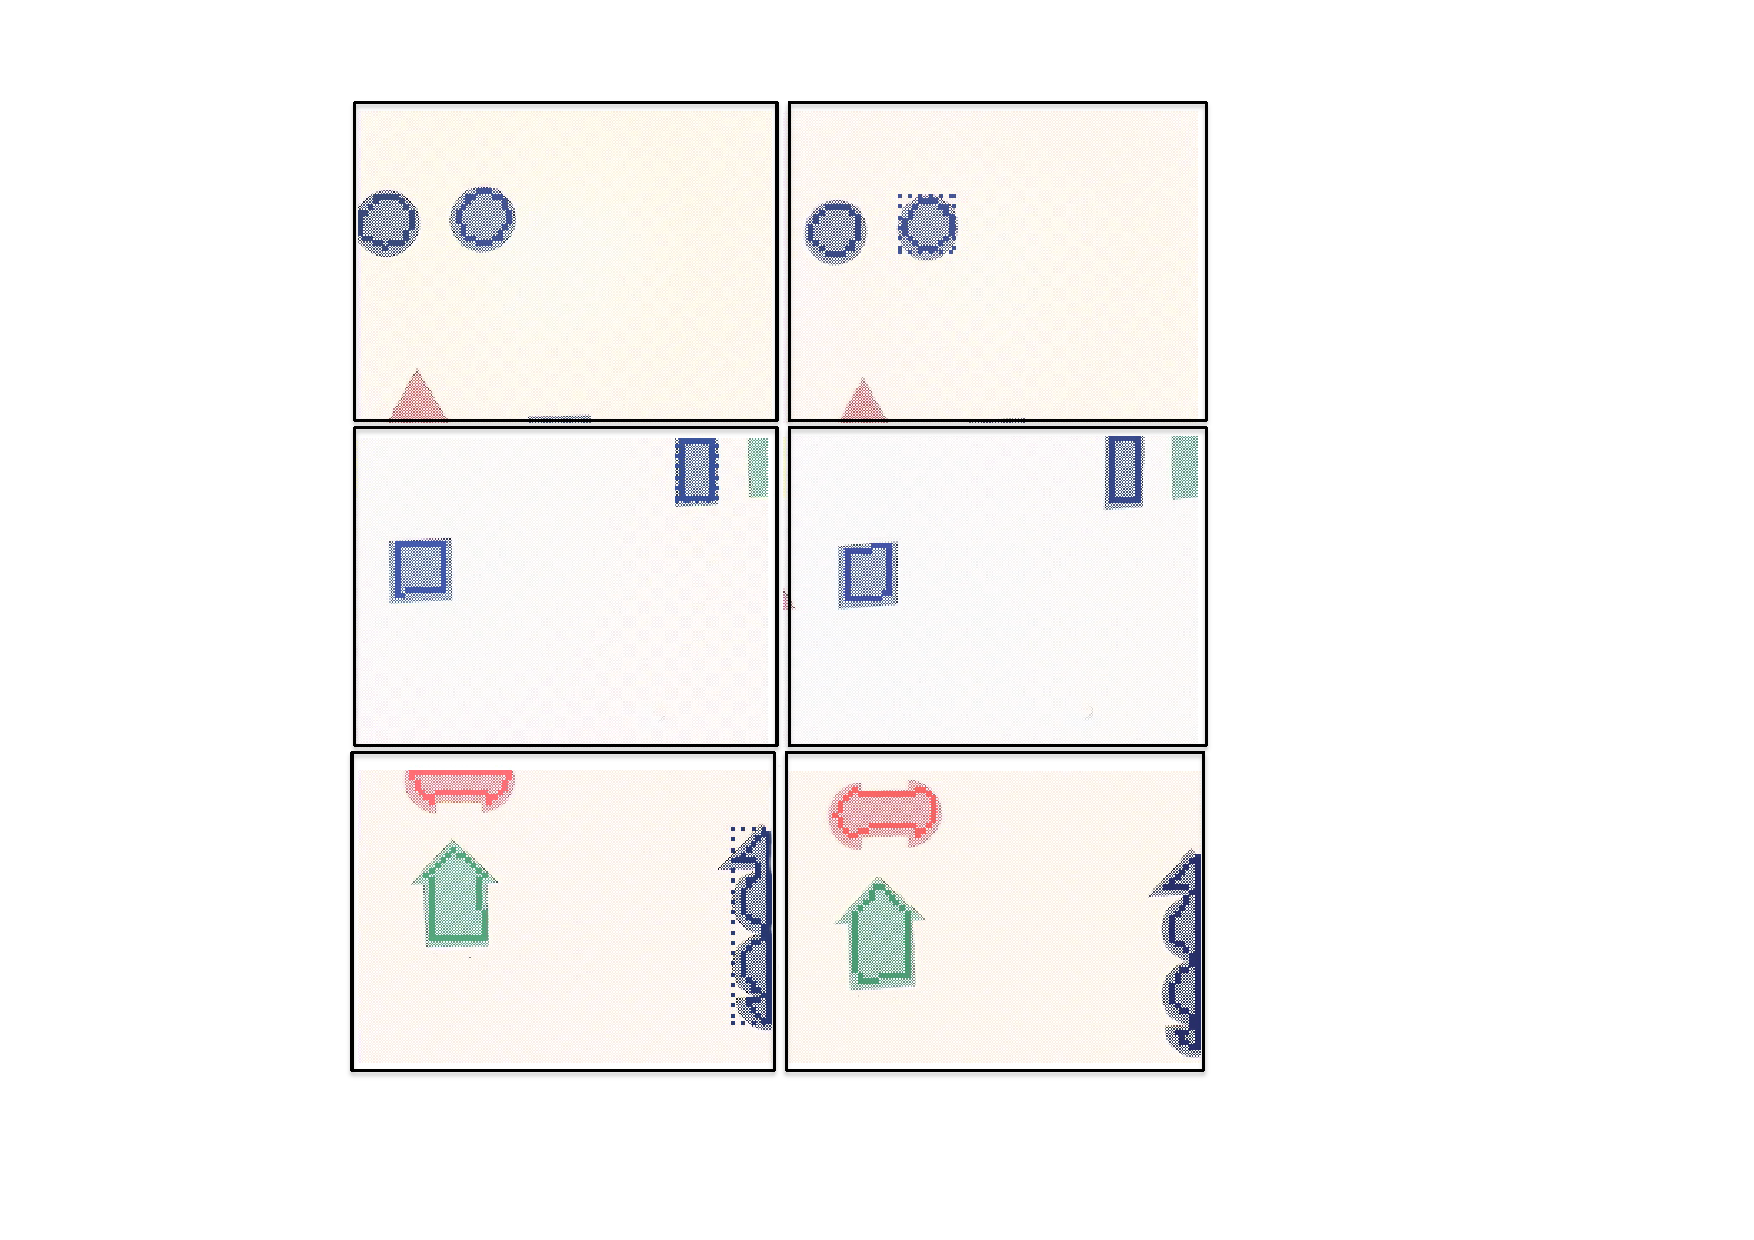
\includegraphics[width=.60\textwidth]{chap2/figs/hpos}}
\caption{ Three examples of segmented images (from top to bottom). Left and right images 
show the perceived and segmented images for two agents respectively. These images are always
different because they are dependent on the position of the agent. 
The topic is indicated by a dashed bounding box in the 
image of the speaker (on the right for the first case and on the left for the others). 
Segments which are too small are ignored. The topics have all been conceptualised
as being `to the right' and so the same word 
"gofubo" has been used to successfully refer to them.}
\label{f:plate10}
\end{figure}

Segmentation can happen according to several criteria. \is{image segmentation}
For example, patches with similar colour can be grouped 
into a single patch, edges can be identified 
and then linked with each other to form line segments
circumscribing the contours of 
an object, or consecutive images can be compared to extract the parts
that changed and hence moved as a single object. 
There is now a solid body of techniques from decades
of machine vision research to efficiently segment scenes according to 
these and other methods. The Talking Heads use several methods
in parallel and combine their output to get a clearly segmented
picture.\footnote{
For general introductions to these areas, 
see: \cite{Ballard:1982} and \cite{Fischler:1987}}

The hearer must be able to sense in which direction the speaker is looking. 
This facility is at the moment implemented by having 
the speaker indicate to the hearer the point on the white board 
at which its camera is focused. The hearer then moves the camera
to this point and records an image as well. The hearer segments 
this image (see \figref{f:plate10}, top image on the left) so that 
now both the speaker 
and the hearer have a set of segments and can start playing 
a language game. Note that the speaker and hearer never get 
exactly the same image because they are standing about one 
meter apart from each other before the white board. Also the
calibration is never entirely accurate so that perceptual 
differences are unavoidable.

\subsection{Sensory Channels}

Next low level visual processes gather information about each \is{sensory channels}
segment, such as its average colour, size, shape,
the position with respect to horizontal or vertical axes. 
Each process outputs its information on a {\it sensory 
channel} scaled between 0.0 and 1.0. The mechanisms from 
the conceptualisation layer that subsequently use this information
can operate on any kind of sensory channel. 
I will assume for the rest of this chapter that the low level
routines produce each only three types of information, sent
on the following sensory channels: 
\begin{itemize}
\item The first channel is called HPOS (horizontal position). 
It contains the x-midposition of a segmented object within
the field of view of the robot. 
\item The second channel is called VPOS (vertical position). It
specifies the y-midposition of the segmented object. 
\item The third channel is called GRAY and contains 
the average gray-scale of the object. 
\end{itemize}
Later on additional channels will be introduced. 

Consider the two objects in \figref{scene1-1}. The triangular
object has the (scaled) values HPOS=0.35, VPOS=0.40, GRAY=0.33, and 
the rectangular object has the values HPOS=0.70, VPOS=0.85, 
GRAY=0.33. The agents can already visually distinguish
millions of possible scenes with these three sensory
channels. The number of scenes
quickly grows when the set of sensory channels increases. 
\begin{figure}[htbp]
  \centerline{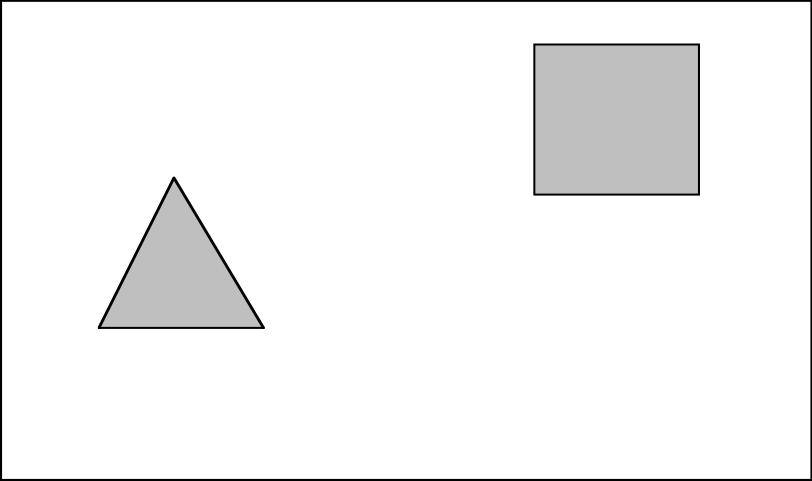
\includegraphics[width=.50\textwidth]{chap2/figs/scene1-1}}
\caption{\label{scene1-1} The scene contains two 
objects: a triangular object and a rectangular object
with the same gray levels. 
Each one is characterised by values on three sensory 
channels: HPOS, VPOS, and GRAY.}
\end{figure}

The low level visual processes outputting
values on the various sensory channels are already quite
complicated in themselves. I will discuss them further in 
chapter 3. I will then argue that the 
agent's repertoire of visual processes does not have to be
static and programmed in advance but evolves and adapts
through a selectionist process. New processes may `grow'
by the random combination of primitive operations and are
pruned when they fail to yield useful information or information 
which is irrelevant in the environment in which the agent 
finds himself. 

\subsection{Making Distinctions}

The data on sensory channels are values from a continuous domain
(between 0.0 and 1.0). 
To be the basis of natural language communication, these
values must be transformed into a discrete domain. This is 
precisely the task of the conceptual layer. It 
performs massive data reduction to make infinitely
rich environments managable. One means of categorization
is to divide up each domain of values on a particular
sensory channel into regions and 
simply assign a category to each region, thus creating a 
discrimination tree.\is{discrimination tree} For example, 
the HPOS-channel can be cut in two halves leading to a 
distinction between [LEFT] ($0.0 \leq HPOS < 0.5$) and [RIGHT] 
($0.5 \leq HPOS \leq 1.0$). The triangular object 
in \figref{scene1-1} has the value HPOS=0.35 
and would therefore be categorized as [LEFT]. Similarly, the 
VPOS-channel can be divided in two halves yielding the 
categories [LOWER] and [UPPER], and likewise the GRAY-channel
yielding the categories [LIGHT] and [DARK]. 
Given these categories, 
the rectangular object in the scene of 
\figref{scene1-1} would be categorized as [RIGHT UPPER LIGHT].
Of course, light, dark, left, lower, etc. are labels 
that I have given to these categories. The Talking Heads 
create categories by partitioning sensory channels but do
not use these labels internally. 

It is always possible to refine a distinction by further
subdividing its region. Thus an agent could further divide the 
bottom region of the HPOS-channel (categorized as 
[LEFT]) into two subregions [TOTALLY-LEFT] ($0.0 \le HPOS < 0.25$), 
and [MID-LEFT] ($0.25 \le HPOS < 0.5$). The triangular object
can now be categorized as [MID-LEFT], if simply categorising it
as [LEFT] is not distinctive enough. Each of these categories can 
still be further refined. The categorisation networks
resulting from these consecutive binary subdivisions form
discrimination trees (\figref{tree1}). It is not at
all assumed that all agents have the same trees; due to 
different developmental histories, divergence is inevitable. 
\begin{figure}[htbp]
  \centerline{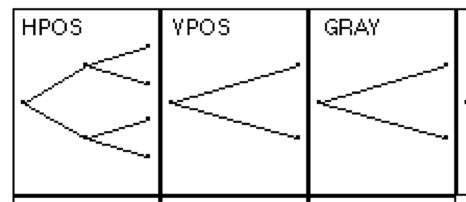
\includegraphics[width=.35\textwidth]{chap2/figs/tree1}}
\caption{\label{tree1} A discrimination tree displays
the divisions of the total range of 
values on a sensory channel into finer and finer subregions. 
Categories are assigned to each region at different 
levels of the tree.}
\end{figure}

There are obviously other ways to 
move from the continuous domain of sensory channels to 
the discrete domain of categories.\footnote{
See: \cite{Taylor:1989}}
For example, it is not really necessary 
to have a binary division, we could just as well split 
each region into three or more subregions. Or we could introduce
focal (prototypical) values and associate
a category with each of them. In the latter case, 
the categorisation process consists 
in identifying the prototype that is closest to 
an object's value. For the current experiment, I will stick however
to a binary categorisation strategy because that is
the simplest to understand and formally investigate. 

We will see that agents build hundreds,
even thousands, of categories as they play their
language games, and in addition they make combinations of 
categories. To bring some order in this profusion of 
categories, I will label them using the 
sensory channel from which a category operates, 
followed by the upper and lower bound of the region they 
carve out. Thus [TOTALLY-LEFT]
is labeled as [HPOS 0.0-0.25], because it carves 
out a region between 0.0 and 0.25 on the HPOS-channel. 
When it must be emphasised that 
a category belongs to a particular agent, for example {\bf a1}, we
write [HPOS 0.0-0.25]$_{\bf a1}$. The same category in agent {\bf a2}
is labeled as [HPOS 0.0-0.25]$_{\bf a2}$. If I want to talk about 
this category in the abstract, I will not mention any 
agent and simply write [HPOS 0.0-0.25]. We will also 
allow conjunctive combinations of categories which will be
written as a set, as in \{[HPOS 0.0-0.25], [VPOS 0.0-0.25]\}, 
which could be paraphrased as totally-left {\it and}
totally-down.  

Where do an agent's discrimination trees, and hence
categories, come from? This is one of the main 
puzzles to be addressed in this book and it will 
occupy most of chapter 4. Very briefly, 
I propose again a selectionist approach, as for
the formation of low level visual routines. I hypothesise
that the nodes and branches of the discrimination trees
grow more or less randomly in all directions. The use and
success of categories is monitored and categories which 
are not sufficiently useful or successful in the environments
encountered by the agent are pruned. I will argue in chapter 4
that this mechanism indeed leads to 
a repertoire of distinctions that is adequate for 
playing language games, and that 
categories therefore need not be innate nor learned by 
induction from a large series of examples. 

\section{Lexicalisation}

Verbalisation (mapping meaning to form) 
involves two distinguishable activities. \is{verbalisation} The first one
relies on a lexicon to map components of meaning to
individual words. The second 
one relies on syntactic rules to provide supra-word structuring 
and additional syntactic marking to express additional
aspects of meaning, particularly how component meanings
are combined into a complex whole. Both types of 
activities also take place in interpretation (mapping form to meaning):
the individual words are mapped back to their meanings
and the meaning of the whole is reconstructed from the 
meaning of the parts. 

In the early origins of language,
there must have been an initial phase in which no complex syntax 
was in place yet. Utterances then must have consisted of single words
or multiple words without further syntax. \is{proto-language}
Such syntax-less languages have been called {\it proto-languages}.\footnote{
See \cite{Bickerton:1990} as well as \cite{Thomason:1988}. Children similarly 
go through a single word phase (even though a single 
word for them might be multiple words for us), and 
then slowly start to bootstrap their grammar. 
See: \cite{Tomasello:1991} and \cite{Bates:1991}. 
They are still observed in the very first phases of 
child language acquisition or in pidgins that spontaneously 
form when two communities with widely diverging languages
need to interact. Out of proto-languages, languages 
with a fully-fledged syntax must have emerged at some point. 
How this occurred is still a heavily debated mystery. In this volume 
I only treat the origins of proto-languages.} 

Children acquire their first words around the first year
of life.\footnote{
Representative work in the study of child language
learning focuses mostly on the acquisition of specific meanings.
See: \cite{Gleitman:1994}, 
\cite{Clark:1993}, \cite{Bowerman:1996}.}
Most people believe that they do this 
as a result of hearing a particular word repeated several times in a
certain context and gradually abstracting an
association between a word and a meaning. But 
how is it that they know which meaning to associate with a 
particular word? How is it that word acquisition goes
so rapid? We will follow a different 
approach, which leaves an open question whether
this applies to human word acquisition as well. The
approach will be selectionist. The agents {\it construct} 
hypotheses, either on the basis of one specific case 
where they guess through a non-verbal strategy what 
the meaning of an unknown word might be, 
or they have simply invented a new word because
they do not have one yet. The hypotheses are 
then tried out in subsequent games and either receive confirmation
or are falsified. As a side effect of this local behavior, 
a global self-organising dynamic process arises leading gradually to coherence. 

Here are a few example games to give a general 
flavor of this selectionist approach to word acquisition. 
Let us assume that there are only two 
agents, {\bf a1} and {\bf a2}, and they use only the 
three sensory channels introduced earlier: VPOS for 
vertical position, HPOS for horizontal position, and GRAY
for grayscale. 

\subsection{Same meaning, same referent}

Here is the simplest possible instance of a
language game, based on the scene in \figref{scene1-1}. 
The speaker, {\bf a1}, has picked the triangle as the topic.
To give a verbal hint, he needs 
to conceptualise this topic, which means in this 
specific case, to find a 
category (or set of categories) which distinguishes the 
topic from the other objects in the context. Here 
the context contains only one additional 
object, namely the rectangle. The category
[VPOS 0.0-0.5]$_{\bf a1}$ (lower) fits the criteria. 
[VPOS 0.0-0.5] is valid when $VPOS < 0.5$
which is the case for the triangle but not for the rectangle. 
{\bf a1} has an association in his lexicon 
relating [VPOS 0.0-0.5]$_{\bf a1}$ with the word "lu", 
{\bf a1} retrieves this word and transmits it to 
the hearer, which is agent {\bf a2}. 

{\bf a2} has stored in his lexicon an
association between "lu" and [VPOS 0.0-0.5]$_{\bf a2}$, and so
hypothesises that [VPOS 0.0-0.5]$_{\bf a2}$ must be the meaning of "lu". 
When this category is applied to the present scene, in other words,
when {\bf a2} filters out the objects whose value for VPOS do not 
fall in the region $[0.0-0.5]$, only one 
remaining object is obtained, the triangle. Hence {\bf a2} concludes that 
this must be the topic and points to it. 

The speaker recognises that the hearer has pointed
to the right object and so the game succeeds. The complete
dialog is reported by the commentator as follows: 
\begin{verbatim}
Game 125.
 a1 is the speaker. a2 is the hearer. 
 a1 segments the context into 2 objects
 a1 categorizes the topic as [VPOS 0.0-0.5]
 a1 says:  "lu"
 a2 interprets "lu" as [VPOS 0.0-0.5]
 a2 points to the topic 
 a1 says: "OK" 
\end{verbatim}
This game illustrates a situation 
where the speaker and the hearer associate the same meaning
with the same form and where the meaning 
picks out the same referent for both agents. No wonder
the game succeeds. Unfortunately things are seldom that simple. 

\subsection{A new word}

There are (at least) two ways in which a game similar to game 125, 
but played earlier might have failed. First of all it can be that
the speaker does not have a word yet for the meaning he wants
to convey. The speaker then invokes a strategy 
to repair this failure. The simplest strategy is to 
create a new word for the present meaning. This is how 
{\bf a1} might have created the word ``lu", and associated it 
with [VPOS 0.0-0.5] in his lexicon. Such simple constructive steps cause
new words to enter the lexicon. 

Second, it can be that the hearer does not know the word. The 
game then fails and the speaker points to 
the topic so that the hearer can make 
an educated guess what the meaning might have been:
If the hearer is able to recover a possible topic
from the non-verbal hint given by the speaker, 
he himself can seek a distinctive category or set of categories 
that delineates this topic from the other objects in 
the context just as the speaker has done. It is 
possible (although not necessary as we will see)
that the hearer {\bf a2} arrives at his 
own version of the same category, namely [VPOS 0.0-0.5]$_{\bf a2}$. The 
hearer now stores in his lexicon a new association between the 
form heard, ``lu", and the guessed meaning [VPOS 0.0-0.5]$_{\bf a2}$. 
Based on this extended lexicon, he will succeed in the same game 
in the future and he can use ``lu" himself to verbalise [VPOS 0.0-0.5]$_{\bf a2}$
when talking to other agents. This is the way new words
spread in the population.

A game where these two repair activities have taken
place is reported by the commentator as follows: 
\begin{verbatim}
Game 25.
 a1 is the speaker. a2 is the hearer. 
 a1 segments the context into 2 objects
 a1 categorizes the topic as [VPOS 0.0-0.5]
 a1 creates a new word: "lu"
 a2 does not know "lu"
 a2 says: "lu?"
 a1 points to the topic 
 a2 categorizes the topic as [VPOS 0.0-0.5]
 a2 stores "lu" as [VPOS 0.0-0.5]
\end{verbatim}

\subsection{Competition between words}

The observant reader will have noticed immediately that 
I have swept some important difficulties under the carpet. 
First, it could very well be that unknown to the speaker 
another agent had already used the word ``lu" 
for another meaning, so that there are now 
two alternative meanings for ``lu" in the lexicon. ``lu" 
has become ambiguous. Second, it may be the hearer {\bf a2} already 
had a word for [VPOS 0.0-0.5]$_{\bf a2}$, for example ``bomida", 
so that there are now two synonyms for [VPOS 0.0-0.5] in the lexicon. 
Synonymy and ambiguity are very common in 
natural languages and unavoidable when a group of 
distributed autonomous agents creates a language without
a central co-ordinator. This implies that 
the agents' lexicon must be sophisticated enough 
to support multiple associations. An agent must be able to 
store the different meanings being used for the same word, and the 
different words being used for the same meaning. 

Will this process not lead to a proliferation of words and 
massive, inefficient lexicons, particularly in large
populations? No. As I will discuss extensively 
in chapter 5, a positive feedback 
loop between use and success
can be set up causing progressive convergence towards an 
efficient lexicon. The agents keep track of the use and 
success of each form-meaning pair and prefer the forms that have had
the most success in past use. The more success a form has, the more
it will be chosen 
and consequently the more success it will have in the 
future. This positive feedback loop creates a winner-take-all 
situation because as soon as one form is slightly preferred, 
its success grows and overtakes its competitors
to eventually dominate (\figref{competition1}). Particularly 
in open environments, the dominance may only be temporary 
after which a new struggle develops and another word 
becomes the winner. 
\begin{figure}[htbp]
  \centerline{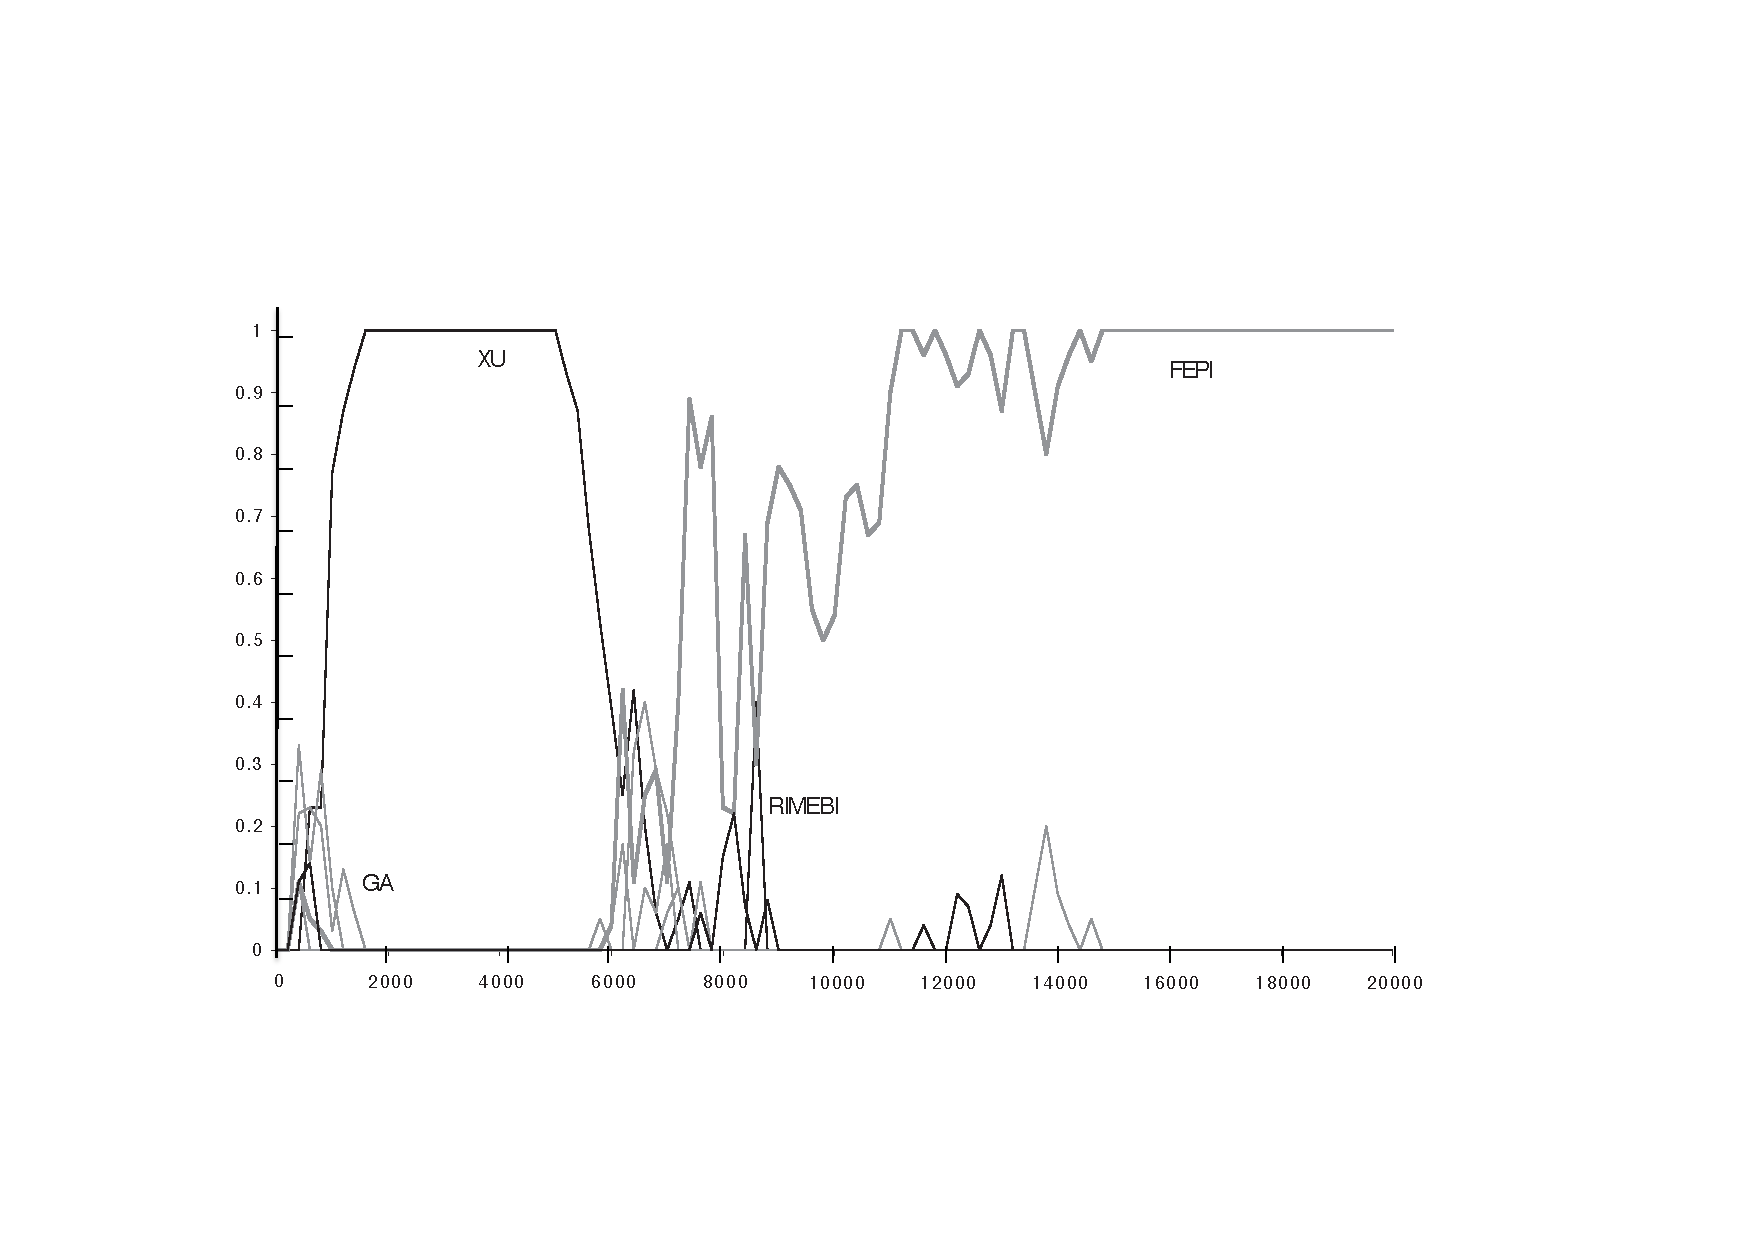
\includegraphics[width=.80\textwidth]{chap2/figs/competition-1}}
\caption{\label{competition1} 
The graph shows the competition between different forms for
expressing one meaning in a population of 20 agents. The graph plots 
the frequency of each form in the population, more precisely the percentage
of agents that prefer a particular word. A complex dynamic
process unfolds with periods where one word (first ``xu" and then ``fepi") dominates.} 
\end{figure}

\subsection{Disambiguation}

Another difficulty which I did not deal with when discussing game 25 above,
is that the hearer may conceptualise
the scene differently from the speaker. For example, 
the triangular object is not only located at the lower half
of the scene and the rectangle at the upper half, 
but it is also to the left, i.e. with $HPOS < 0.5$, whereas
the rectangle is to the right. It follows that the 
hearer could just as well have hypothesised that ``lu" means [HPOS 0.0-0.5] (left)
and not [VPOS 0.0-0.5] (lower). 

Is this bad? It depends on the situations being encountered
in the future. When the game is played again for the
same scene with {\bf a1} saying ``lu" to mean [VPOS 0.0-0.5], and 
{\bf a2} interpreting ``lu" as [HPOS 0.0-0.5], the game would succeed! 
Communicative success is achieved whenever the 
hearer recovers the referent chosen by the 
speaker; it is not required that they 
use exactly the same meaning. In fact, the hearer can never know
for sure what meaning was initially conceptualised by the speaker and 
neither can the speaker know which meaning was understood 
by the hearer because they cannot look inside each
other's head. The meaning can be quite different, 
as we have just seen, as long as it is compatible. 

Even more remarkably, if a topic which is at the lower
portion of the scene, is always 
on the left side and vice-versa, there would always be 
success despite the different meanings of ``lu", 
and the players would never discover
that each means something else by ``lu". 

Similar situations arise in human natural language communication
as well, particularly for words
which are not stabilised yet or whose interpretation 
depends strongly on the non-verbal information provided
by the context. They also arise when the speaker or hearer
have different sensory modalities or sensibilities. 
For example, a colour-blind person (unable to 
make the distinction between red and green) will recognise
the red traffic light by its position. For that person, 
``stop for the red light" does not mean stop for 
the light that has the colour red but stop when the 
upper-most light is lit. 

These examples show clearly that shared language and meaning 
arise from the efforts of agents to co-ordinate their
conceptualisations and lexicalisations with respect 
to the environments they encounter and the games they play, 
but that these co-ordinations cannot be perfect nor totally 
uniform because the agents have limited rationality. 
In general, we can {\it not} assume that different agents
have exactly the same 
conceptualisation of reality and that they mean the same thing by 
the same words. As we will see in later experiments, the
Talking Heads hardly agree on the meaning of a word, particularly 
in the early phases of language development, but they 
nevertheless manage to have a surprisingly high communicative success
rate. There is no guarantee that a particular 
form maps onto the same meaning, even in the same language community.
Despite these shaky foundations, communication is generally 
successful because there is sufficient coherence among the members of 
a community and sufficient constraints from the context. 

\begin{figure}[htbp]
  \centerline{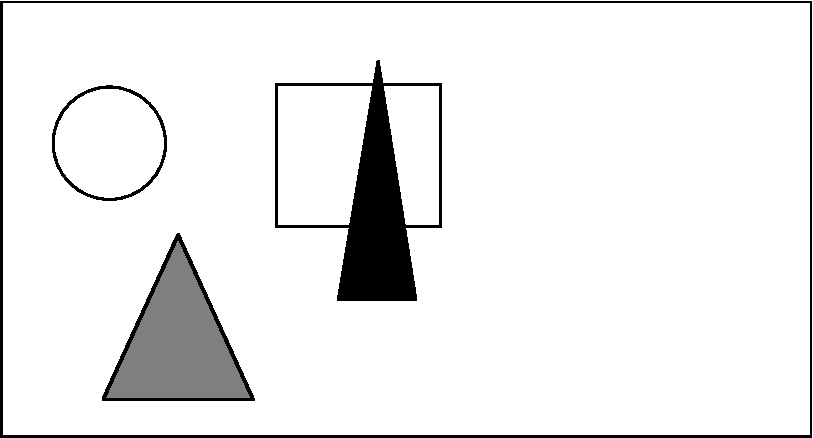
\includegraphics[width=.50\textwidth]{chap2/figs/scene1-2}}
\caption{\label{scene1-2} A second scene which 
can be used to disambiguate ``lu".}
\end{figure}
Consider now another scene (\figref{scene1-2}). The speaker
is again {\bf a1} and categorizes the bottom triangle as 
[VPOS 0.0-0.5]$_{\bf a1}$, meaning
the object at the lower half of the scene. Assuming that the
hearer {\bf a2} has associated ``lu" with [HPOS 0.0-0.5]$_{\bf a2}$, he
would interpret ``lu" as [HPOS 0.0-0.5]$_{\bf a2}$ (to the left). But this 
does not yield a single 
referent and therefore the game fails. 
This failure is an opportunity for the hearer to repair his 
hypotheses about the possible meanings of "lu".
When he conceptualises the scene himself, 
he finds that [VPOS 0.0-0.5]$_{\bf a2}$ distinguishes the triangle
from the circle. A new association between 
"lu" and [VPOS 0.0-0.5]$_{\bf a2}$ is stored. The old association
is not removed but enters in competition with the new
one, and gradually one meaning will come to dominate
by the winner-take-all mechanism discussed earlier on. 

The commentator reports this kind of interaction as follows: 
\begin{verbatim}
Game 137.
 a1 is the speaker. a2 is the hearer. 
 a1 segments the context into 4 objects
 a1 categorizes the topic as [VPOS 0.0-0.5]
 a1 says:  "lu"
 a2 interprets "lu" as [HPOS 0.0-0.5]
 There is more than one such object
 a2 says: "lu?"
 a1 points to the topic
 a2 categorizes the topic as [VPOS 0.0-0.5]
 a2 stores "lu" as [VPOS 0.0-0.5]
\end{verbatim}

Through such disambiguating situations, meanings of words
get clarified and the lexicons of the agents
become more similar. Note that the 
dominating meaning of ``lu" can still go in 
two directions. For example, {\bf a2}
could have used ``lu" with {\bf a1} 
in a situation where its only possible meaning 
is [HPOS 0.0-0.5] (left). Then {\bf a1}, now playing the role
of hearer, would have stored the association between
``lu" and [HPOS 0.0-0.5]. If this happened often 
enough [HPOS 0.0-0.5] (left) might
have become the dominant meaning of ``lu", instead of 
[VPOS 0.0-0.5] (lower). This shows clearly that the 
evolution of language will never be predictable. At a critical 
bifurcation, small preferential differences between 
the agents or the chance occurrence of certain situations
may tilt the competition in one direction or the other.\footnote{
This high sensitivity to initial conditions is 
one of the characteristics of a chaotic dynamic
system \cite{Lorenz:1993}.
Indeed, as I will explore in more detail later, 
evolving languages have all the characteristics
of complex adaptive systems, including the 
potential for punctuated equilibria.}
There is no right
or wrong solution in the language game and no one has
any more rights than anyone else. 

\subsection{Same meaning, different referent} 

When agents have the same meaning for the same
form, it is likely that they
pick out the same referent from the context. When agents
have a different meaning for the same form, it is less 
likely although it may still happen that they pick 
out the same referent, as we have seen. But there 
is an even more problematic situation: When agents have the 
same meaning for the same form but nevertheless pick out 
different referents! 

For example, suppose that two Talking Heads have developed the 
concept of [LEFT] and [RIGHT] with respect to their own position 
in front of the scene. In terms of the sensory 
channels we have been using, anything to the left of their field  
of vision ($0.0 \le HPOS < 0.5$) is categorized as
left, i.e. [HPOS 0.0 0.5], and everything right  
($0.5 < HPOS \le 1.0$) is categorized as right, 
i.e. [HPOS 0.0 0.5]. But because the
agents stand next to each other and have therefore 
slightly different positions with respect to the 
scene in front of them, there is an area which will 
be categorized as right for one head and left for the other (\figref{left-right})
\begin{figure}[htbp]
  \centerline{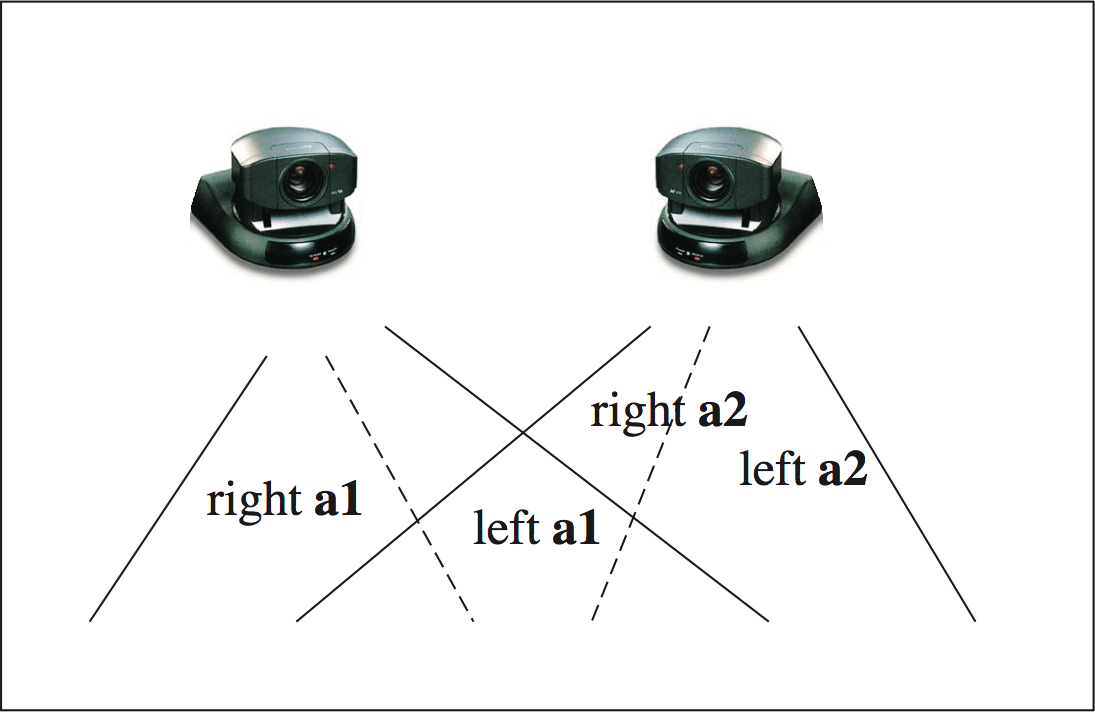
\includegraphics[width=.65\textwidth]{chap2/figs/left-right}}
\caption{\label{left-right} Two talking heads are shown {\bf a1} and 
{\bf a2} each seeing the scene from a slightly different viewpoint.}
\end{figure}
When this occurs in real dialogs, the form-meaning 
pairs lexicalising the distinctions left and right destabilise,
because sometimes it gets positive feedback as 
it succeeds in the game, and at other times it 
gets negative feedback. 
This is one of the reasons why human categories are often 
relative and scaled with respect to a context.
For example, we say ``the triangle to the left of the square", in 
other words left with respect to the square, to avoid the uncertainty
inherent in the absolute use of ``left". Humans scale the size 
of objects with respect to the scene, so that small 
objects are small compared to the others in the scene 
and not small in an absolute sense. 

\subsection{Situated grounded semantics}

These various examples, and I am clearly only \is{situated grounded semantics}
scratching the surface, already illustrate the major thrust of the 
approach explored in more detail in the remainder of this book. 
There are dynamic processes at two levels. (1) There is 
the evolution of a lexicon in a single agent: new words are
invented or adopted from another agent and the
scores of form-meaning pairs in the lexicon
go up and down depending on success or
failure in the game. At any point in time, an agent 
will have a preferred form to express a particular meaning, 
but he has also stored the alternative words floating around in the 
population, and his preference will change depending on feedback
in further language games. (2) There is also lexicon evolution at 
the level of the group. A coherent global lexicon emerges because
the lexicons of the individual agents become more and more 
similar. This is due to the positive feedback loop between
the outcome of using
a certain form-meaning pair and the probability that
this pair will be used again in the future. 
The group lexicon will however seldom be exactly uniform because
new meanings constantly pop up and agents may arrive from 
other language communities, bringing in new words. 
I will study this two level dynamic process in much more detail 
in chapter 7. It explains many of the mysteries of
language, for example why there is ambiguity. 

The `semantic theory' required to make the 
Talking Heads experiment work is very different from 
the classical textbook approaches to the subject, which
tend to assume that categories can be defined in the 
abstract, independent of their context of use. Grounded
conceptualisation and interpretation processes are necessarily 
strongly situated and context-dependent. Whether ``blue 
triangle" is going to be effective in picking out the 
intended topic depends on what else is in
the scene. If all other objects in the 
context are also blue triangles, the game will fail. If there
is only one triangle, it was not really necessary to say that 
it is blue. This situatedness and context-dependence, together with 
the non-verbal hints given by the speaker, are crucial 
keys for restricting the 
possible meanings of a form 
and they therefore help the hearer disambiguate 
utterances or figure out the meaning of an unknown form. But situatedness 
and context-dependence are also major
sources of difficulty, because the same categories may
refer to different things for different agents in different
contexts. Even if both agents agree that a particular form 
names a certain category, 
they may still fail in the game if the category picks
out a different referent, for example because they see 
the context from a slightly different vantage point. 

Another major difference with classical theories of 
meaning and reference is 
that the repertoire of meanings and form-meaning pairs is open-ended
and subject to change at any time. Logicians would say that the 
truth conditions of the forms are non-monotonic. \is{non-monotonicity}
Non-monotonicity is unavoidable in the case of grounded 
situated agents with limited rationality.\footnote{
Examples of these processes are described in: 
\cite{Bybee:1994}, \cite{Traugott:1991}.
For attempts to explain these "grammaticalization" 
processes in terms of general cognitive operations, see: 
\cite{Heine:1997}.}
Agents should always be allowed to 
introduce new forms or recruit existing forms to express new
meanings, simply because the set of meanings must expand
to cope with novel contexts and new communicative
situations. After enough interactions among the 
members of the same group in a relatively stable 
environment, we expect there to be
a stable set of conventionalised form-meaning 
relations, but it cannot be
expected that everything anyone ever wants to say is
already conventionalised, and so there will always
be turbulence at the fringes. The idea that the lexicon
and the syntax of a language are static
entities is completely false. Both are in constant flux.
Non-monotonicity is consequently one of the big 
topics in logic-based approaches to artificial intelligence.

A theory of language must try 
to capture the strategies by which language users shape and 
reshape their language and by which some solutions may become 
conventionalised and spread in the rest of the population, 
rather than focus on describing the end results of 
this process. This open-ended adaptive character of 
language systems is explored extensively in chapter 7. 

This section probably raised many questions in the 
mind of the critical reader: Will the agents really 
reach a sufficiently similar lexicon to have successful 
communication, despite the fact that no one has a 
complete overview nor controls globally what the others
can say? Are the unclear situations, i.e. those
where more than one possible meaning is possible, not 
going to destabilise existing lexicons? Will all this 
scale up both for the size of the agent set and for 
the size of the meaning set? Is a new, virgin agent 
going to be able to catch up with a lexicon already 
existing in a population? What happens when two 
populations each with their own entrenched lexicon meet? 
These are exactly the kinds of questions that I will 
address later. They can all be posed in a precise 
way within the context of the Talking Heads experiment.

\section{The origins of grammar}

The self-organisation of a shared lexicon in a population
of agents already represents a formidable challenge.
We need to find models that work in principle {\it and} 
we have to make them operational on physically 
instantiated autonomous robots. 
But many linguists would claim that this does not yet 
represent true language, they would want to see the 
emergence of a genuine syntax. How that might
happen is one of the ultimate remaining scientific
mysteries of our time but let me sketch a possible approach. 

Basically, I hypothesise that the agents must 
first of all have the capability to generate much 
more complex semantic and pragmatic strategies for conceptualising
reality or applying a conceptualisation to retrieve 
a referent.

For example, a phrase like "the two red
triangles to the left of the smallest green square" requires
the following strategy: 
\begin{enumerate}
\item The agent filters the set of possible objects in 
the scene to retain only the squares. 
\item He further filters the resulting set to retain only 
the green ones. 
\item He orders the remaining green squares based on 
size and then picks out the smallest one. 
\item Then he orders the objects in the scene based on 
their horizontal position (HPOS) and retains only those
whose position is to the left of the smallest green square. 
\item From the remaining set he filters out the triangles, 
and from this set those with a red colour. 
\item This final set should contain only two members
and they constitute the referents of the original phrase. 
\end{enumerate}
Our research has already lead to  
mechanisms whereby agents can autonomously generate such
semantic strategies using processes that compose
primitive strategies into complex ones. The
strategies compete for use in language games. 
New strategies form when needed by the environment or 
the agent's interactions and those that do not work or 
are irrelevant get pruned. The mechanisms for generating 
and selecting such semantic strategies are not unique
to language. The invention and use of tools or the 
planning of a series of actions and the retrieval 
and use of ready-made plans requires exactly the 
same sorts of capabilities. 

The spontaneous generation of repertoires of complex 
semantic strategies already explains some characteristics 
that are reflected in full-fledged languages: 
There is hierarchical structure, because one strategy 
may call upon another strategy to achieve a subgoal, 
and a strategy may potentially call upon itself thus introducing 
recursivity. There is also a functional specialisation
of categories. They are now sometimes used for filtering
the members of a set, sometimes for ordering them, sometimes
for modifying another category before it is used for 
filtering, and so on. Hierarchical structuring, recursivity
and functional specialisation therefore do not have to 
originate in language. The fact that we see them in 
language structure is a reflection of the generic 
hierarchical and functional nature 
of semantic strategies.\footnote{
The fact that languages change is, of course, 
well-known in linguistics even though it is less a focal 
research topic than used to be in the 19th century. 
See: \cite{McMahon:1994} for a brief introduction into the 
subject. Language change has many of the characteristics
of biological change but it takes place in cultural 
as opposed to biological time. See: \cite{Labov:1994}}. 

Second, my hypothesis is that the need for communicating 
more and more complex semantic strategies and the 
conceptual structures they use, has pushed language 
users to start using more and more complex form characteristics, 
starting with word order but also intonation, stress 
patterns, function words, morphological variations of words, 
etc. Here another aspect comes into 
play: the ability to recognise forms and structures, 
which we also need to recognise structured objects in 
scenes for example, and the ability to assemble a 
structure satisfying a set of constraints. The collective
dynamics which are responsible for the propagation and the spontaneous 
self-organisation of coherence in lexicons should also apply  
here. Grammars can be seen as ecologies, where
form-meaning pairs compete in the population. New 
syntactic and semantic categories, new constructions and 
new uses of grammatical conventions are continuously created,
and existing ones may destabilise and become
in disuse.\footnote{
The semantic strategies are similar to the 
cognitive processes that have been studied extensively 
in cognitive grammar \cite{Langacker:1987}. Formal versions
of some of these processes have been formulated as 
part of Montague grammar \cite{Montague:1974}. In 
computational linguistics research, various 
attempts have been made to formalise conceptualisation
and meaning application strategies. \cite{Gazdar:1989}}

Each language user employs his own ideolect which is 
as well as possible co-ordinated with that of other
language users but there is never complete similarity 
and never absolute stability.  
This explains perhaps why linguists have such a hard
time to pin down ``the" language of a community. As soon 
as someone speaks, language changes. 

According to this theory, natural language structure is
not the consequence of an 
autonomous innate language device which evolved 
by a genetic mutation or series of mutations. Instead 
cognitive mechanisms and structures already in place have been 
marshalled to get a language system off the ground, even though 
once language became essential for the rapid incorporation
of new individuals and the general organisation of 
activities in human populations, it must have started
to recruit vast amounts of brain capacity and stimulated 
other cognitive faculties, such as categorisation,
episodic memory or problem solving, to become in turn 
much more complex and versatile.\footnote{
There has been an ongoing nature versus nurture debate 
with respect to the origins and acquisition of language. 
The different issues in this debate are already well
illustrated in \cite{Piattelli:1980}.} 

Before the problem of syntax can 
be tackled seriously, we must have a solid foundation showing 
how agents are capable of autonomously acquiring individual words
or combinations of words without syntax. This is the subject of the
remainder of the present volume.

\section{Conclusions}

The Talking Heads experiment examines with what kinds
of mechanisms physically embodied autonomous agents 
might be capable of bootstrapping an ontology, a lexicon, 
and a syntax. The Talking Heads are situated embodied
agents. This 
allows them to build up and co-ordinate language and meaning 
in tight interaction with a shared physical environment
as perceived through their cameras. 
The Talking Heads are social agents, members of a
language community. The collective
dynamics of the community is a crucial ingredient to understanding
how successful communications of a similar complexity as
human natural language communications might have 
originated and how the underlying system can 
be maintained from one generation to the next. 

This chapter has described the main hardware 
and software components of the agents and briefly sketched
their internal architecture. The operation and effect
of this architecture have been 
illustrated with some example games. The remaining chapters explore the 
various aspects of the agent's capacities in much more detail. 
First I will break the global task down into different subtasks, 
as suggested by the semiotic square. We will start by looking how agents 
may establish the relation between a real world object and 
a segmented image (chapter 3). Then we study how they 
relate a segmented image to its conceptualisation (chapter 4). 
Third, we study how a conceptualisation can be related to 
an utterance (chapter 5). In chapter 6 and 7 we couple these
various components and study the lexical and ontological 
dynamic processes that result. 

%\end{document}

